\documentclass{standalone}

\usepackage{graphicx}

\usepackage{tikz}

\usetikzlibrary{positioning}
\usetikzlibrary{arrows.meta}

\begin{document}

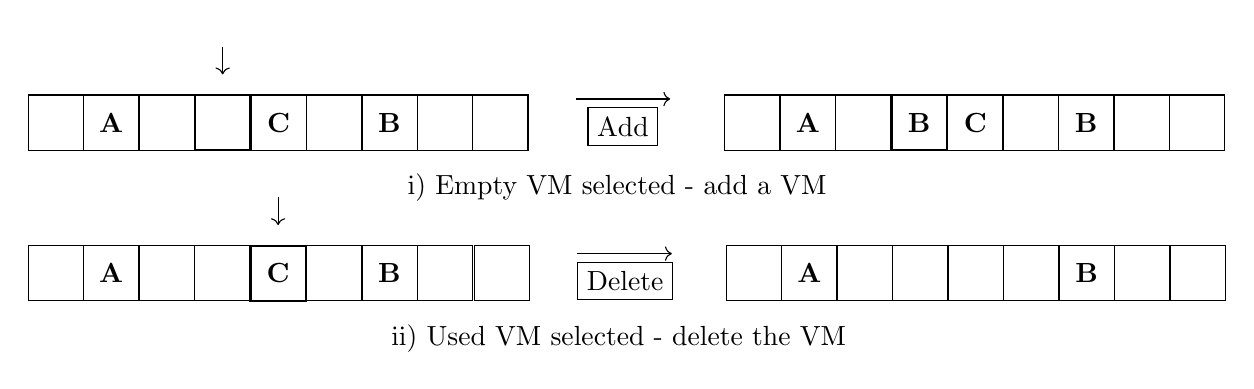
\begin{tikzpicture}[
    cell/.style={rectangle, draw, minimum width=.7cm, minimum height = .7cm},
]

% Add mutation
\node[cell] (BA1) {};
\node[cell] (BA2) [right= -.01cm of BA1] {\textbf{A}};
\node[cell] (BA3) [right= -.01cm of BA2] {};
\node[cell] (BA4) [right= -.01cm of BA3, thick] {};
\node[cell] (BA5) [right= -.01cm of BA4] {\textbf{C}};
\node[cell] (BA6) [right= -.01cm of BA5] {};
\node[cell] (BA7) [right= -.01cm of BA6] {\textbf{B}};
\node[cell] (BA8) [right= -.01cm of BA7] {};
\node[cell] (BA9) [right=-.01cm of BA8] {};

\node (H1) [right=1cm of BA9] {};
\node (H2) [below=-0.2cm of H1] {};

\node (T1) [draw, rectangle, right=-.5cm of H2] {Add};

\node (HA1) [above=.1cm of H2] {};

\node (A1) [left=.4cm of HA1] {};
\node (A2) [right=1.2cm of A1] {};

\draw[->] (A1) -- (A2);

\node (H2) [right=1cm of H1] {};

\node[cell] (BD1) [right=-.01cm of H2] {};
\node[cell] (BD2) [right=-.01cm of BD1] {\textbf{A}};
\node[cell] (BD3) [right=-.01cm of BD2] {};
\node[cell] (BD4) [right=-.01cm of BD3, thick] {\textbf{B}};
\node[cell] (BD5) [right=-.01cm of BD4] {\textbf{C}};
\node[cell] (BD6) [right=-.01cm of BD5] {};
\node[cell] (BD7) [right=-.01cm of BD6] {\textbf{B}};
\node[cell] (BD8) [right=-.01cm of BD7] {};
\node[cell] (BD9) [right=-.01cm of BD8] {};

\node (A3) [above=.6cm of BA4] {};
\node (A4) [above=0cm of BA4] {};
\draw[->] (A3) -- (A4);

\node (C1) [below=.4cm of H1] {i) Empty VM selected - add a VM};

% Delete mutation
\node[cell] (BD1) [below = 1.2cm of BA1] {};
\node[cell] (BD2) [right= -.01cm of BD1] {\textbf{A}};
\node[cell] (BD3) [right= -.01cm of BD2] {};
\node[cell] (BD4) [right= -.01cm of BD3] {};
\node[cell] (BD5) [right= -.01cm of BD4, thick] {\textbf{C}};
\node[cell] (BD6) [right= -.01cm of BD5] {};
\node[cell] (BD7) [right= -.01cm of BD6] {\textbf{B}};
\node[cell] (BD8) [right= -.01cm of BD7] {};
\node[cell] (BD9) [right=--.01cm of BD8] {};

\node (HD1) [right=1cm of BD9] {};
\node (HD2) [below=-0.15cm of HD1] {};

\node (TD1) [draw, rectangle, right=-.65cm of HD2] {Delete};

\node (HAD1) [above=.1cm of HD2] {};

\node (AD1) [left=.4cm of HAD1] {};
\node (AD2) [right=1.2cm of AD1] {};

\draw[->] (AD1) -- (AD2);

\node (HD2) [right=1cm of HD1] {};

\node[cell] (AD1) [right=-.01cm of HD2] {};
\node[cell] (AD2) [right=-.01cm of AD1] {\textbf{A}};
\node[cell] (AD3) [right=-.01cm of AD2] {};
\node[cell] (AD4) [right=-.01cm of AD3] {};
\node[cell] (AD5) [right=-.01cm of AD4] {};
\node[cell] (AD6) [right=-.01cm of AD5] {};
\node[cell] (AD7) [right=-.01cm of AD6] {\textbf{B}};
\node[cell] (AD8) [right=-.01cm of AD7] {};
\node[cell] (AD8) [right=-.01cm of AD8] {};

\node (AD3) [above=.6cm of BD5] {};
\node (AD4) [above=0cm of BD5] {};
\draw[->] (AD3) -- (AD4);

\node (C2) [below=.4cm of HD1] {ii) Used VM selected - delete the VM};

\end{tikzpicture}

\end{document}